\documentclass[../../thesis.tex]{subfiles}


\begin{document}
\begin{figure}[p]
    \centering
    \pgfdeclarelayer{bg}    % declare background layer
    \pgfsetlayers{bg,main}  % set the order of the layers (main is the standard layer)
    \subfloat[]{
    \tikzsetnextfilename{wafer_296_transmission}
    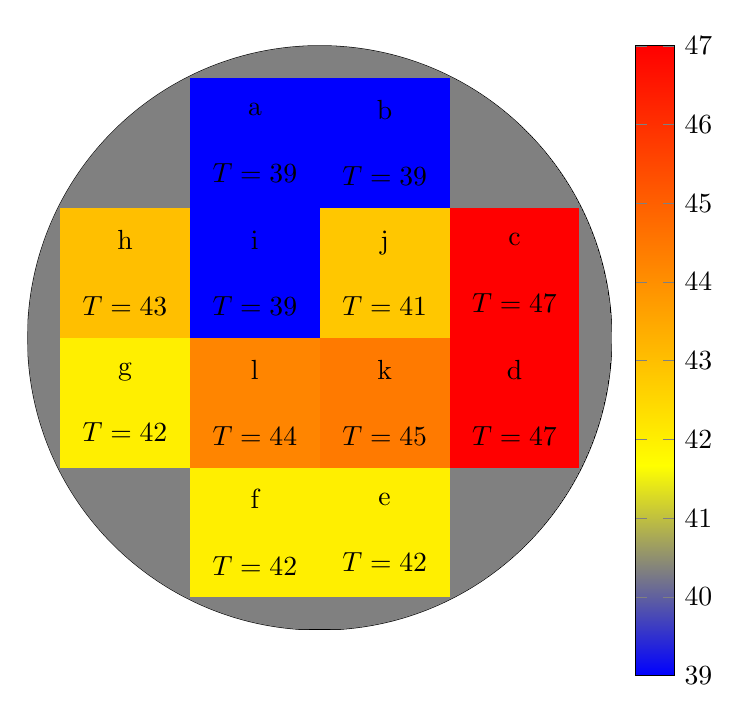
\begin{tikzpicture}
      \tikzset{
        jet/.style={
        },
    }
        \begin{scope}[xshift=-4.5cm,yshift=-4cm]
        \begin{axis}[
            hide axis,
            colormap/hot,
            xmin=-4.5, xmax=4.5,
            ymin=-4.5, ymax=4.5,
            axis equal,
            width=9cm,
            height=9cm,
            colorbar,
            point meta min=39,
            point meta max=47,
            colorbar style={
              width=0.5cm,
              height=8cm,
              xtick={39,41,...,47}}
        ]
            \clip[draw] (0,-0) circle (4.5);
            \fill[gray] (0,-0) circle (4.5);
            \fill[/utils/exec={\pgfplotscolormapdefinemappedcolor{500}}, color of colormap=0] (-2,4) -- (0,4) -- (0,2) -- (-2,2) -- cycle;
            \node[align = center] at (-1,3) {a\\ \\ $T = \SI{39}{\percent}$};
            %b
            \fill[/utils/exec={\pgfplotscolormapdefinemappedcolor{500}}, color of colormap=0] (0,4) -- (2,4) -- (2,2) -- (-0,2) -- cycle;
            \node[align = center] at (1,3) {b\\ \\ $T = \SI{39}{\percent}$};
            %c
            \fill[/utils/exec={\pgfplotscolormapdefinemappedcolor{500}}, color of colormap=1000] (2,2) -- (2,0) -- (4,0) -- (4,2) -- cycle;
            \node[align = center] at (3,1) {c\\ \\ $T = \SI{47}{\percent}$};
            %d
            \fill[/utils/exec={\pgfplotscolormapdefinemappedcolor{500}}, color of colormap=1000] (2,0) -- (4,0) -- (4,-2) -- (2,-2) -- cycle;
            \node[align = center] at (3,-1) {d\\ \\ $T = \SI{47}{\percent}$};
            %e
            \fill[/utils/exec={\pgfplotscolormapdefinemappedcolor{500}}, color of colormap=375] (0,-2) -- (2,-2) -- (2,-4) -- (0,-4) -- cycle;
            \node[align = center] at (1,-3) {e\\ \\ $T = \SI{42}{\percent}$};
            %f
            \fill[/utils/exec={\pgfplotscolormapdefinemappedcolor{500}}, color of colormap=375] (-2,-2) -- (0,-2) -- (0,-4) -- (-2,-4) -- cycle;
            \node[align = center] at (-1,-3) {f\\ \\ $T = \SI{42}{\percent}$};
            %g
            \fill[/utils/exec={\pgfplotscolormapdefinemappedcolor{500}}, color of colormap=375] (-4,0) -- (-2,0) -- (-2,-2) -- (-4,-2) -- cycle;
            \node[align = center] at (-3,-1) {g\\ \\ $T = \SI{42}{\percent}$};
            %h
            \fill[/utils/exec={\pgfplotscolormapdefinemappedcolor{500}}, color of colormap=500] (-4,2) -- (-2,2) -- (-2,0) -- (-4,0) -- cycle;
            \node[align = center] at (-3,1) {h\\ \\ $T = \SI{43}{\percent}$};
            %i
            \fill[/utils/exec={\pgfplotscolormapdefinemappedcolor{500}}, color of colormap=0] (-2,2) -- (0,2) -- (0,0) -- (-2,0) -- cycle;
            \node[align = center] at (-1,1) {i\\ \\ $T = \SI{39}{\percent}$};
            %j
            \fill[/utils/exec={\pgfplotscolormapdefinemappedcolor{500}}, color of colormap=480] (0,2) -- (2,2) -- (2,0) -- (0,0) -- cycle;
            \node[align = center] at (1,1) {j\\ \\ $T = \SI{41}{\percent}$};
            %k
            \fill[/utils/exec={\pgfplotscolormapdefinemappedcolor{500}}, color of colormap=680] (0,0) -- (2,0) -- (2,-2) -- (0,-2) -- cycle;
            \node[align = center] at (1,-1) {k\\ \\ $T = \SI{45}{\percent}$};
            %l
            \fill[/utils/exec={\pgfplotscolormapdefinemappedcolor{500}}, color of colormap=650] (-2,0) -- (0,0) -- (0,-2) -- (-2,-2) -- cycle;
            \node[align = center] at (-1,-1) {l\\ \\ $T = \SI{44}{\percent}$};
            \draw[step=2] (-4.5,-4.5) grid (4.5,4.5);
        \end{axis}
        \end{scope}
      \end{tikzpicture}
      \label{fig:296-transmission}}
      \\
      \subfloat[]{
      \tikzsetnextfilename{wafer_295_transmission}
      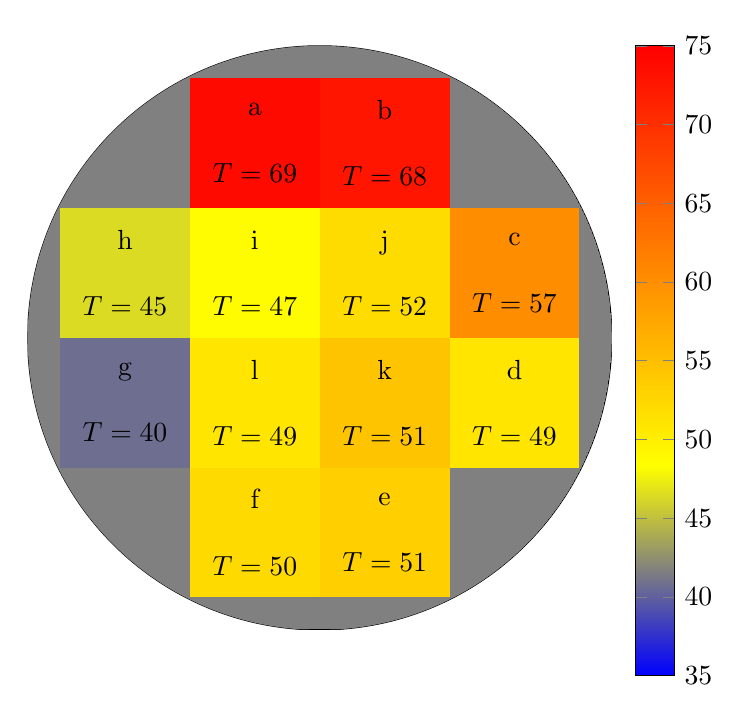
\begin{tikzpicture}
        \begin{scope}[xshift=-4.5cm,yshift=-4cm]
          \begin{axis}[
              hide axis,
              colormap/hot,
              xmin=-4.5, xmax=4.5,
              ymin=-4.5, ymax=4.5,
              height=9cm,
              width=9cm,
              axis equal,
              colorbar,
              point meta min=35,
              point meta max=75,
              colorbar style={
                width=0.5cm,
                height=8cm,
                xtick={35,40,...,70}
              }
          ]
              \clip[draw] (0,-0) circle (4.5);
              \fill[gray] (0,-0) circle (4.5);
              \fill[/utils/exec={\pgfplotscolormapdefinemappedcolor{500}}, color of colormap=971] (-2,4) -- (0,4) -- (0,2) -- (-2,2) -- cycle;
              \node[align = center] at (-1,3) {a\\ \\ $T = \SI{69}{\percent}$};
              %b
              \fill[/utils/exec={\pgfplotscolormapdefinemappedcolor{500}}, color of colormap=942] (0,4) -- (2,4) -- (2,2) -- (-0,2) -- cycle;
              \node[align = center] at (1,3) {b\\ \\ $T = \SI{68}{\percent}$};
              %c
              \fill[/utils/exec={\pgfplotscolormapdefinemappedcolor{500}}, color of colormap=629] (2,2) -- (2,0) -- (4,0) -- (4,2) -- cycle;
              \node[align = center] at (3,1) {c\\ \\ $T = \SI{57}{\percent}$};
              %d
              \fill[/utils/exec={\pgfplotscolormapdefinemappedcolor{500}}, color of colormap=400] (2,0) -- (4,0) -- (4,-2) -- (2,-2) -- cycle;
              \node[align = center] at (3,-1) {d\\ \\ $T = \SI{49}{\percent}$};
              %e
              \fill[/utils/exec={\pgfplotscolormapdefinemappedcolor{500}}, color of colormap=457] (0,-2) -- (2,-2) -- (2,-4) -- (0,-4) -- cycle;
              \node[align = center] at (1,-3) {e\\ \\ $T = \SI{51}{\percent}$};
              %f
              \fill[/utils/exec={\pgfplotscolormapdefinemappedcolor{500}}, color of colormap=429] (-2,-2) -- (0,-2) -- (0,-4) -- (-2,-4) -- cycle;
              \node[align = center] at (-1,-3) {f\\ \\ $T = \SI{50}{\percent}$};
              %g
              \fill[/utils/exec={\pgfplotscolormapdefinemappedcolor{500}}, color of colormap=143] (-4,0) -- (-2,0) -- (-2,-2) -- (-4,-2) -- cycle;
              \node[align = center] at (-3,-1) {g\\ \\ $T = \SI{40}{\percent}$};
              %h
              \fill[/utils/exec={\pgfplotscolormapdefinemappedcolor{500}}, color of colormap=286] (-4,2) -- (-2,2) -- (-2,0) -- (-4,0) -- cycle;
              \node[align = center] at (-3,1) {h\\ \\ $T = \SI{45}{\percent}$};
              %i
              \fill[/utils/exec={\pgfplotscolormapdefinemappedcolor{500}}, color of colormap=343] (-2,2) -- (0,2) -- (0,0) -- (-2,0) -- cycle;
              \node[align = center] at (-1,1) {i\\ \\ $T = \SI{47}{\percent}$};
              %j
              \fill[/utils/exec={\pgfplotscolormapdefinemappedcolor{500}}, color of colormap=425] (0,2) -- (2,2) -- (2,0) -- (0,0) -- cycle;
              \node[align = center] at (1,1) {j\\ \\ $T = \SI{52}{\percent}$};
              %k
              \fill[/utils/exec={\pgfplotscolormapdefinemappedcolor{500}}, color of colormap=486] (0,0) -- (2,0) -- (2,-2) -- (0,-2) -- cycle;
              \node[align = center] at (1,-1) {k\\ \\ $T = \SI{51}{\percent}$};
              %l
              \fill[/utils/exec={\pgfplotscolormapdefinemappedcolor{500}}, color of colormap=400] (-2,0) -- (0,0) -- (0,-2) -- (-2,-2) -- cycle;
              \node[align = center] at (-1,-1) {l\\ \\ $T = \SI{49}{\percent}$};
              \draw[step=2] (-4.5,-4.5) grid (4.5,4.5);
            \end{axis}
          \end{scope}
        \end{tikzpicture}
        \label{fig:295-transmission}}
      \caption{Transmission measurements of wafer 296 \protect\subref{fig:296-transmission} and wafer 295 \protect\subref{fig:295-transmission}. Wafer 296 has been measured in untreated closed pore state. The membranes 295a and 295b are closed pore membranes while the rest of wafer 295 has been opened.}
      \label{fig:wafer-transmission}
\end{figure}
\end{document}
